\documentclass[12pt,a4paper]{article}

\usepackage[utf8]{inputenc}
\usepackage[T1]{fontenc}
\usepackage[a4paper,margin=3cm]{geometry}
\usepackage{amsmath}
\usepackage{array}
\usepackage{booktabs}
\usepackage{caption}
\usepackage{graphicx}
\usepackage{hyperref}
\usepackage{url}

\hypersetup{
    colorlinks=true,
    linkcolor=black,
    urlcolor=blue,
    citecolor=black
}

\setlength{\emergencystretch}{2em}
\setlength{\parskip}{0.5em}
\setlength{\parindent}{0pt}
\linespread{1.08}

\newcommand{\mdp}{Maximum Diversity Problem}
\newcommand{\grasp}{GRASP}
\newcommand{\graspTS}{GRASP+TS}
\newcommand{\tabu}{Tabu Search}

\title{\textbf{GRASP and Tabu Search for the Maximum Diversity Problem}}
\author{Carlos Gomez Saez \and Raul Rodriguez Gomez}
\date{Data Based Logistics -- May 2026}

\begin{document}

\maketitle

\begin{abstract}
This project studies the \mdp{} using the classroom \grasp{} framework as baseline and a \grasp{} combined with \tabu{} as the proposed method. The main contribution is not a generic description of metaheuristics, but an implementation and experimental comparison of a short-term memory search procedure on the original MDG instances. The final data show that both methods tie on the small instances, while \graspTS{} clearly improves the baseline on the large instances under the calibrated parameters and the same time budget.
\end{abstract}

\section{Introduction}

The goal of the project is to solve the \mdp{} with metaheuristics and to evaluate whether adding \tabu{} improves the \grasp{} method used as reference in class. \tabu{} was chosen as the project extension instead of Path Relinking. The report focuses on the implemented method, the calibration decisions, and the computational evidence.

The final comparison uses the 15 original MDG-a instances: 6 small instances with \(n=100\), \(m=10\), and 9 large instances with \(n=500\), \(m=50\). All runs are time-limited, so the comparison is based on equal wall-clock conditions rather than a fixed number of iterations.

\section{Problem Description}

Given \(n\) elements and pairwise distances \(d_{ij}\), the \mdp{} asks for a subset \(S\) of exactly \(m\) elements maximizing the sum of distances between all selected pairs:

\begin{equation}
\max \sum_{i<j} d_{ij} x_i x_j,
\qquad
\sum_i x_i = m,
\qquad
x_i \in \{0,1\}.
\end{equation}

The problem is a maximization problem. In the experiments, the reference value \(BK\) is the best value observed in the current runs for each instance. Relative deviation is computed as:

\begin{equation}
\mathrm{Dev} = \frac{BK - \mathrm{MethodValue}}{BK}\cdot 100.
\end{equation}

Lower deviation is better. A deviation of \(0\%\) means that the method reached the best observed value for that instance.

\section{Baseline GRASP}

The baseline is the \grasp{} structure provided in class: each restart builds a solution with a greedy-randomized construction and then applies local search. The construction uses a Restricted Candidate List controlled by the parameter \(\alpha\). Low values of \(\alpha\) are greedier; high values are more random. The value \(\alpha=-1\) means that the construction samples a random alpha value.

Most of the original classroom structure is preserved: instance reading, solution representation, incremental objective updates, constructive logic, and the multi-start organization. The important change is the local search used in the final baseline. The classroom version selected the element with the smallest contribution and searched for its best replacement. The current version evaluates all selected/non-selected one-out one-in swaps and applies the best positive delta. Therefore, the baseline is a strengthened \grasp{}, not a weak reference method.

\section{Tabu Search Method}

The proposed method is \graspTS{}. Each restart first generates an initial solution using the same \grasp{} construction. Then \tabu{} improves that solution while respecting the remaining global time budget.

The move is a one-out one-in exchange: one selected node leaves the solution and one non-selected node enters. The neighborhood is complete: at each iteration, the algorithm scans all selected/non-selected pairs and chooses the best admissible move. Unlike standard improving local search, \tabu{} can accept worsening moves. This is necessary to leave local optima and explore new regions.

The implementation keeps two tabu memories:

\begin{itemize}
    \item \texttt{tabu\_out}: nodes recently removed from the solution cannot immediately re-enter;
    \item \texttt{tabu\_in}: nodes recently inserted into the solution cannot immediately leave.
\end{itemize}

This bidirectional memory avoids simple cycles. The tabu tenure is dynamic: in each iteration it is sampled between the calibrated tenure and approximately \(1.5\) times that value. A tabu move can still be accepted by aspiration if it improves the best global solution. The algorithm stops when the time limit is reached or after a maximum number of iterations without improvement. The best global solution is stored separately and returned at the end.

The implemented \graspTS{} loop can be summarized as follows:

\begin{enumerate}
    \item Build an initial feasible solution with the GRASP constructive phase.
    \item Initialize the current solution and the best global solution.
    \item Scan all one-out one-in swaps and select the best admissible move.
    \item If a move is tabu, accept it only if it satisfies aspiration.
    \item Apply the move, update the current objective value, and update both tabu lists.
    \item If the current solution improves the best global value, store a copy of it.
    \item Stop when the time budget or the no-improvement limit is reached.
\end{enumerate}

\section{Implementation Details}

Solutions are represented as Python dictionaries with a set of selected nodes, the current objective value, and a pointer to the instance. The selected nodes are stored in a \texttt{set}, which makes membership checks efficient during neighborhood scans.

The objective function is updated incrementally. When a node leaves the solution, its marginal contribution is subtracted; when a node enters, its contribution to the remaining selected set is added. This avoids recomputing the full pairwise sum after every move.

The main implementation decisions were:

\begin{itemize}
    \item use the same construction logic for both methods, so the comparison isolates the improvement phase;
    \item strengthen the \grasp{} baseline with exhaustive best-improvement local search;
    \item use complete one-out one-in neighborhoods in both local search and \tabu{};
    \item implement bidirectional tabu memory with readable FIFO lists instead of a more complex data structure;
    \item pass the remaining global time from the \graspTS{} wrapper to the internal \tabu{} phase;
    \item record convergence information whenever a new global best is found inside \tabu{}.
\end{itemize}

The main difficulties were time control and avoiding misleading convergence plots. A first version only registered the value after a whole \tabu{} phase, hiding improvements that happened inside it. The final version logs internal improvements with their elapsed time.

Another important decision was how to keep the code close to the classroom baseline. The project did not rewrite the instance format, the constructive procedure, or the solution operations. This makes the final comparison easier to interpret: the main experimental question is whether replacing the improvement phase with \tabu{} adds value.

Results are stored in CSV files so the same data can be used for tables, statistical tests, Excel exports, and plots. The final comparison stores both aggregate rows per instance and individual paired runs. This was necessary for the Wilcoxon test, because stochastic runs should be compared by matched seed index instead of only by global averages.

\section{Parameter Calibration}

Calibration was performed before the final comparison. The tested values were:

\begin{itemize}
    \item \(\alpha \in \{0.1, 0.25, 0.5, 0.75, 0.9, -1\}\);
    \item tabu tenure \(\in \{5, 10, 15, 20, 25, 30\}\).
\end{itemize}

The calibration used 10 seconds per run and 3 runs per configuration. The criterion was average relative deviation. The \graspTS{} calibration was sequential: first \(\alpha\) was tested with tenure fixed at 15, and then tenure was tested using the selected \(\alpha\).

\begin{table}[htbp]
\centering
\caption{Selected calibrated parameters.}
\begin{tabular}{lccc}
\toprule
Group & \(\alpha\) for \grasp{} & \(\alpha\) for \graspTS{} & Tabu tenure \\
\midrule
Small & 0.1 & -1 & 5 \\
Large & 0.1 & 0.1 & 10 \\
\bottomrule
\end{tabular}
\end{table}

Small instances were saturated during calibration, so several configurations reached zero deviation. The large instances were more informative: the selected \graspTS{} setting was \(\alpha=0.1\), tenure \(=10\).

The calibration result is relevant because it prevents an unfair comparison. A poorly chosen tenure can either make \tabu{} cycle too quickly or block useful moves for too long. In the final large-instance setting, tenure \(=10\) gives enough memory to avoid immediate reversals without over-constraining the search.

\section{Computational Results}

The final comparison used 30 seconds per run and 5 paired runs per instance and method. The small instances are fully saturated: all 30 paired runs are exact ties. The large instances show a clear advantage for \graspTS{}.

\begin{table}[htbp]
\centering
\caption{Per-instance final comparison. Average times are in seconds.}
\tiny
\setlength{\tabcolsep}{2pt}
\begin{tabular}{@{}lrrrrrrrr@{}}
\toprule
Instance & BK & G avg & G dev & G time & TS avg & TS dev & TS time & TS hits \\
\midrule
MDG-a\_1\_100\_m10 & 360.15 & 360.15 & 0.0000\% & 30.00 & 360.15 & 0.0000\% & 30.00 & 5 \\
MDG-a\_4\_100\_m10 & 355.72 & 355.72 & 0.0000\% & 30.00 & 355.72 & 0.0000\% & 30.00 & 5 \\
MDG-a\_10\_100\_m10 & 355.50 & 355.50 & 0.0000\% & 30.00 & 355.50 & 0.0000\% & 30.00 & 5 \\
MDG-a\_12\_100\_m10 & 354.25 & 354.25 & 0.0000\% & 30.00 & 354.25 & 0.0000\% & 30.00 & 5 \\
MDG-a\_14\_100\_m10 & 356.06 & 356.06 & 0.0000\% & 30.00 & 356.06 & 0.0000\% & 30.00 & 5 \\
MDG-a\_20\_100\_m10 & 349.31 & 349.31 & 0.0000\% & 30.00 & 349.31 & 0.0000\% & 30.00 & 5 \\
MDG-a\_2\_n500\_m50 & 7741.07 & 7695.50 & 0.5887\% & 30.46 & 7729.77 & 0.1460\% & 30.02 & 1 \\
MDG-a\_5\_n500\_m50 & 7755.23 & 7697.35 & 0.7463\% & 30.34 & 7739.21 & 0.2066\% & 30.02 & 2 \\
MDG-a\_6\_n500\_m50 & 7770.48 & 7712.16 & 0.7505\% & 30.31 & 7754.04 & 0.2116\% & 30.03 & 1 \\
MDG-a\_9\_n500\_m50 & 7758.44 & 7730.84 & 0.3557\% & 30.24 & 7741.52 & 0.2181\% & 30.03 & 1 \\
MDG-a\_13\_n500\_m50 & 7786.43 & 7737.72 & 0.6256\% & 30.35 & 7761.13 & 0.3249\% & 30.02 & 1 \\
MDG-a\_16\_n500\_m50 & 7792.77 & 7739.38 & 0.6851\% & 30.27 & 7756.25 & 0.4686\% & 30.04 & 1 \\
MDG-a\_17\_n500\_m50 & 7785.36 & 7723.03 & 0.8006\% & 30.50 & 7772.74 & 0.1621\% & 30.03 & 2 \\
MDG-a\_19\_n500\_m50 & 7755.41 & 7702.49 & 0.6824\% & 30.46 & 7745.61 & 0.1264\% & 30.02 & 2 \\
MDG-a\_20\_n500\_m50 & 7727.13 & 7688.01 & 0.5063\% & 30.44 & 7712.33 & 0.1915\% & 30.03 & 1 \\
\bottomrule
\end{tabular}
\end{table}

\begin{table}[htbp]
\centering
\caption{Aggregate results on large instances.}
\begin{tabular}{lcc}
\toprule
Metric & \grasp{} & \graspTS{} \\
\midrule
Average deviation & 0.6379\% & 0.2284\% \\
Mean standard deviation & 20.57 & 20.27 \\
Best hits & 0 & 12 \\
Paired wins & 8 & 36 \\
Ties & \multicolumn{2}{c}{1} \\
Mean delta TS--GRASP & -- & +31.7891 \\
Wilcoxon \(p\)-value & -- & \(8.24\cdot 10^{-8}\) \\
\bottomrule
\end{tabular}
\end{table}

Two additional plots were generated to understand the behavior of \tabu{}.

\begin{figure}[htbp]
\centering
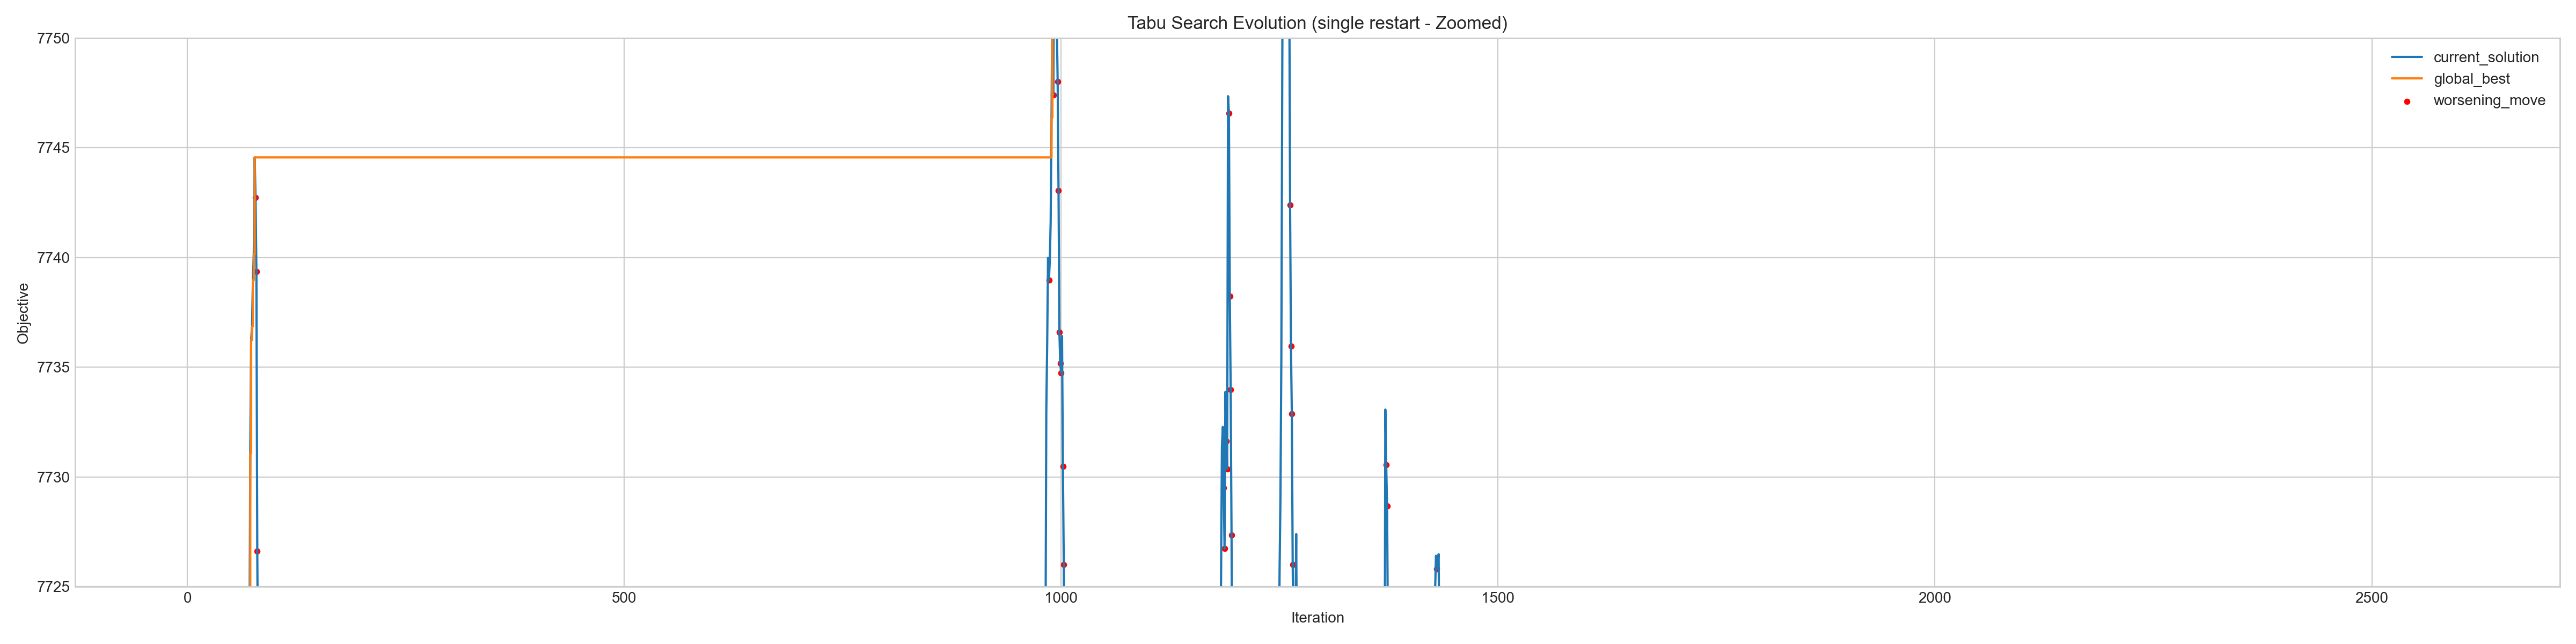
\includegraphics[width=\textwidth]{csv_final/ts_evolution_plot.png}
\caption{Internal evolution of one Tabu Search restart. The current solution can worsen temporarily, while the best global value is non-decreasing.}
\end{figure}

The trace contains 2586 iterations, including 1403 worsening moves. This confirms that the implemented \tabu{} is not just a greedy local search; it actively accepts worsening moves to escape local optima.

\clearpage

\begin{figure}[htbp]
\centering
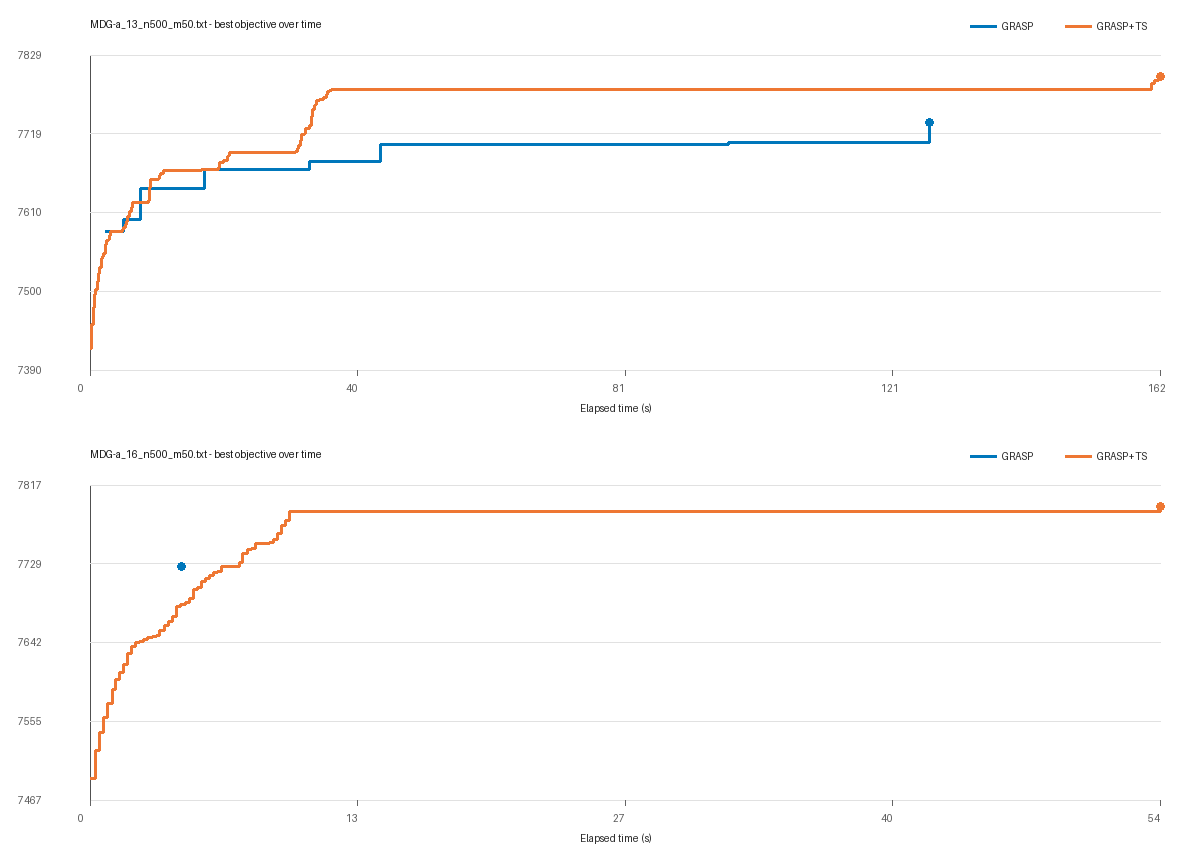
\includegraphics[width=\textwidth]{csv_final/convergence_curves_large.png}
\caption{Convergence over 180 seconds on two large instances.}
\end{figure}

With 180 seconds, \graspTS{} reached 7792.77 on MDG-a\_16 and 7798.43 on MDG-a\_13, while \grasp{} reached 7726.43 and 7734.12 respectively. This supports the same conclusion as the 30-second comparison: deeper tabu intensification is useful on large instances.

\begin{table}[htbp]
\centering
\caption{Long-run convergence values with 180 seconds per algorithm.}
\begin{tabular}{lcc}
\toprule
Instance & \grasp{} final & \graspTS{} final \\
\midrule
MDG-a\_16\_n500\_m50 & 7726.43 & 7792.77 \\
MDG-a\_13\_n500\_m50 & 7734.12 & 7798.43 \\
\bottomrule
\end{tabular}
\end{table}

\section{Discussion}

The results show two different regimes. On small instances, both methods reach the same values. These instances are too easy under a 30-second budget, so \tabu{} adds no measurable benefit.

On large instances, \graspTS{} improves the baseline. It has lower average deviation, more paired wins, and all best hits on the large group. The reason is consistent with the implementation: the large instances leave more room for local optima, and \tabu{} can cross worsening moves while preserving the best global solution.

The improvement is not free. \tabu{} spends more time inside each trajectory and completes fewer independent restarts than plain \grasp{}. For small instances this extra depth is unnecessary. For large instances it pays off because the search space is harder and the memory mechanism helps escape local regions.

The main limitation is that the reference \(BK\) is the best value observed in our runs, not an external optimum. Also, calibration was sequential rather than a full joint grid over \(\alpha\) and tenure. Finally, the implementation tracks node frequencies but does not yet use them as a long-term diversification mechanism.

\section{Conclusions}

\tabu{} is useful in this project, but not uniformly. It does not improve \grasp{} on the small instances because both methods already saturate them. On the large instances, \graspTS{} clearly improves the strengthened \grasp{} baseline under the calibrated parameters and the same time budget.

The most important lesson is that the value of \tabu{} depends on the instance size and on implementation details: complete swap evaluation, bidirectional tabu memory, dynamic tenure, aspiration, and correct time control all matter. With more time, the natural next steps would be a full joint calibration of \(\alpha\) and tenure, a cleaner long-term frequency-based diversification mechanism, and comparison with Path Relinking.

\end{document}
